% !TeX root = ../main.tex
% Add the above to each chapter to make compiling the PDF easier in some editors.

\chapter{Combatting the Precision Loss of Variable Analyses}\label{chapter:precisionLossVariableAnalyses}
  In this chapter we describe our approach to reduce the precision loss described in \autoref{sec:precisionLoss} for analyses tracking information in relation to variables. We call analyses of this kind "variable analyses".\\
  First we use the syntax for flow sensitive analyses from \autoref{chapter:background} to formally explain the idea. After that we explain a concrete implementation of the approach into the \gob\ analyzer.
  \section{Formal description}
  We want to reduce the mentioned precision loss for variable analyses. The basic idea to achieve this, is to track for each procedure which variables have been written or have possibly been altered in some other way within that procedure. This information is then used in variable analyses when combining the abstract state from the caller with the abstract return state given by the callee at the end of the procedure. We will exemplify this with the values-of-variables we introduced in \autoref{chapter:background}.\\
  \\
  In the following we call a variable that has been written or altered in the current procedure context "tainted". Therefore, we introduce a new taint analysis tracking which variables have been tainted within the context of the current procedure in the following section. It is worth mentioning that our notion of taintedness is related but different from other uses of the term "taint analysis".\\
    \subsection{Taint analysis}\label{sec:formalTaint}
      Let us formulate the syntax for the taint analysis we propose in this thesis: Since we want to find a collection of tainted variables per program point, a suitable domain for this analysis is the powerset of the set of variables $X$ ordered by the subset relation:
      \[\mathbb{D}_\textsf{t} = 2^X \text{ with } \sqsubseteq_\textsf{t} = \subseteq\]
      To be compatible with the notion of partially context-sensitive analyses from \autoref{sec:partialCtxSens} we need to also specify a context domain $\mathbb{C}_\textsf{t}$ which we define later.
      Note that we seek to compute a mapping from program points (with context) to sets of variables, i.e., $\eta_\textsf{t}: (N \times \mathbb{C}_\textsf{t}) \rightarrow \mathbb{D}_\textsf{t}$. To interpret this with the goal of our taint analysis in mind, we note that $\eta_\textsf{t} [n, \bullet] = T$ denotes that $T$ is the set of possibly tainted variables at program point $n$. Expressed differently this means that for any variable $x \in T$ we cannot exclude that this variable was altered between the start of the current procedure up until the program point $n$. Note here that the tainted set $T$ not only includes variables which have been tainted by statements of the current procedure, but also variables which have been tainted within procedures called by the current one.\\
      It remains to define $\mathbb{C}_\textsf{t}$, $\textsf{init}^{\#}_\textsf{t}$, $\textsf{enter}^{\#}_\textsf{t}$ and $\textsf{combine}^{\#}_\textsf{t}$ as well as the abstract effects of actions $[\![ A ]\!]^{\#}$. Recall that the notion of a "tainted" variable is defined in relation to the current procedure. This means we want to start without any variable being initially tainted when entering a procedure. It is worth pointing out that the entry to a procedure call does not depend on the state where it is called. Therefore, we design our analysis to be context-insensitive, i.e., 
      \[\mathbb{C}_\textsf{t} = \{\bullet\} \text{ and trivially } \textsf{context}^{\#}_\textsf{t}\ T = \bullet\]
      With these considerations we can also define $\textsf{enter}^{\#}_\textsf{t}$ and $\textsf{init}^{\#}_\textsf{t}$ as follows:
      \[\textsf{enter}^{\#}_\textsf{t}\ T = \textsf{init}^{\#}_\textsf{t} = \emptyset\]
      It is worth pointing out here that the function $\textsf{enter}^{\#}_\textsf{t}\ T$ is always equal to the empty set irregardless of its argument $T$. Therefore, it computes the same entry state for each call of a certain procedure.\\
      When combining the caller state with the returned callee state, we note that we need to keep the tainted set from before the call, as a tainted variable can never get "untainted" again, no matter what the procedure does. Additionally, we add the tainted set returned by the callee, since anything tainted in the call needs to be considered tainted after the call as well. This is because we want to know which variables have been altered in a procedure call, no matter if the tainting happened within the procedure itself or within a further procedure call. This leaves us with the following equation for the $\textsf{combine}^{\#}_\textsf{t}$ function:
      \[ \textsf{combine}^{\#}_\textsf{t}\ (T_\textsf{cr}, T_\textsf{ce}) = T_\textsf{cr} \cup (T_\textsf{ce} \backslash Locals_\textsf{ce}) \]
      Note that we removed the callee local variables $Locals_\textsf{ce}$ because these are not accessible by the caller and all of its callers anyway, so it is not useful to keep track of them.\\
      Lastly we define the abstract effects of actions. Most of these (including checks) do not do anything besides propagating through the state from before. The only major exception are variable assignments. For these we note that the specific variable, which the value is assigned to is added to the tainted set. This is independent of the expression that evaluates to the assigned value, as we are only interested in the fact that the variable on the left of the assignment is altered. This leaves us with the following abstract effects of actions:
      \[ [\![ A ]\!] ^{\#}\ T = \left\{ \begin{array}{ll}
        T \cup \{x\} & \text{if }A \equiv (x = e;)\\
        T & \text{else}
      \end{array} \right. \]
      where $e$ is any arbitrary expression.\\
      This concludes our definition of the taint analysis.

    \subsection{Improving Variable Analyses}\label{sec:formalImprove}
    In this section we see how the information from the taint analysis helps us to improve variable analyses. We show this with the example of the values-of-variables analysis we introduced in \autoref{chapter:background}.\\
    Recall the source of the precision loss we want to reduce as described in \autoref{sec:precisionLoss}. This happened when a global variable was updated with a less precise value after a procedure call even though this specific variable was not changed by the call.\\
    Thanks to the taint analysis we defined in the previous section, we now have a way to get information about which variables can be altered by a procedure $f()$ and which surely stay untouched. The latter of which are exactly those variables which are not in the tainted set of the end node $e_f$ for that procedure.\\
    With this insight we can now update the $\textsf{combine}^{\#}_\textsf{v}$ function of our values-of-variables analysis as follows:
    \[
      \textsf{combine}^{\#}_\textsf{v}\ (M_\textsf{cr}, M_\textsf{ce}) = M_\textsf{cr}|_{Locals_\textsf{cr}\, \cup\, (Globals\, \textbackslash\, T_\textsf{ce})} \oplus M_\textsf{ce}|_{Globals\, \cap\, T_\textsf{ce}}
    \]
    where for an edge $(u, f();, v)$ we have $T_\textsf{ce} = \eta_\textsf{t}\ [e_f, c]$ for the respective context $c$ to be combined.\\
    Similar to before the $\textsf{combine}^{\#}_\textsf{v}$ function takes the caller mapping, restricts it to a subset of caller reachable variables and updates this mapping with the callee mapping restricted to the rest of caller reachable variables. In other words, the caller reachable variables are partitioned into two sets such that one subset is taken from the caller state while the other one is taken from the callee state. Before our change, the partitioning was done strictly in such a way that only the caller local variables were taken from the caller state and all global variables from the callee state. After our improvement, the global variables that are not tainted by the callee are also taken from the caller state and not from the callee anymore. Thereby the precision loss for untainted variables is eliminated.
    \\
    One might wonder if our change could lead to a case, where the callee state has a more precise value for a variable that is discarded because this variable is not in the tainted set. Concretely this situation would be described by 
    \[\exists \text{ Edge }(u, f();, v),\ x \in Globals: x \notin \eta_\textsf{t}\ [e_f, \bullet] \land (\eta_\textsf{v}\ [e_f, \bullet]\ x\subset \eta_\textsf{v}\ [u, \bullet]\ x)\]
    From $x \notin \eta_\textsf{t}\ [e_f, \bullet]$ we know that $x$ has not been altered in the procedure $f()$ since the node $s_f$ up until $e_f$, and therefore it holds that 
    \[\eta_\textsf{v}\ [e_f, \bullet]\ x = \eta_\textsf{v}\ [s_f, \bullet]\ x\]
    Because $x$ is a global we get with the definitions of $\sqsubseteq_\textsf{v}$ and $\textsf{enter}^{\#}_\textsf{v}$: 
    \[\eta_\textsf{v}\ [s_f, \bullet]\ x \supseteq (\textsf{enter}^{\#}_\textsf{v}\ (\eta_\textsf{v}\ [u, \bullet]))\ x = \eta_\textsf{v}\ [u, \bullet]\ x\]
    Therefore, $\eta_\textsf{v}\ [e_f]\ x\supseteq \eta_\textsf{v}\ [u]\ x$ which is a contradiction to the proposed case which we can therefore exclude.

  \section{Implementation}\label{sec:implementation}
  Before explaining the process of implementing the proposed taint analysis and its usage to improve other analyses, we introduce the \gob\ analyzer and its structure in this paragraph. The core functionality of \gob\ is to statically analyze C programs using an approach similar to the one described in \autoref{chapter:background}. This generally works as follows: After the C input file is preprocessed, a \ac{CFG} is generated. This graph is then used together with the specifications of various analyses to generate a constraint system. \gob\ solves this constraint system and produces different kinds of outputs to the user according to the solution (e.g. notifications, warnings or a visualization of the full solution).\\
  It is worth mentioning that \gob\ can perform multiple analyses on a program at the same time. For this a compound domain is built (for the value domain as well as for the context domain), that is a tuple of the domains corresponding to the analyses to be performed. To generate constraints, all activated analyses are taken into account, where the specification of each analysis acts on its corresponding part of the compound domain. Information can be transferred between the different analyses via a system called "queries".\\
  % TODO: Improve:
  \autoref{fig:gob_structure_detail} shows the inner structure of the analyzer. We can see that \gob\ provides parametrized domains which can be used in the specifications of the analyses, e.g., \texttt{Set} and \texttt{Map}. It is also shown that multiple analyses are then compounded into one Master Control Program (MCP) that is used by the framework to generate constraints from the \ac{CFG}. The resulting constraint system is then solved by one of the solvers \gob\ provides in \texttt{/solvers}.\\  
  For a deeper insight into the inner workings of \gob\ refer to \parencite{apinis2014frameworks}.
  
  \begin{figure}
    \centering
    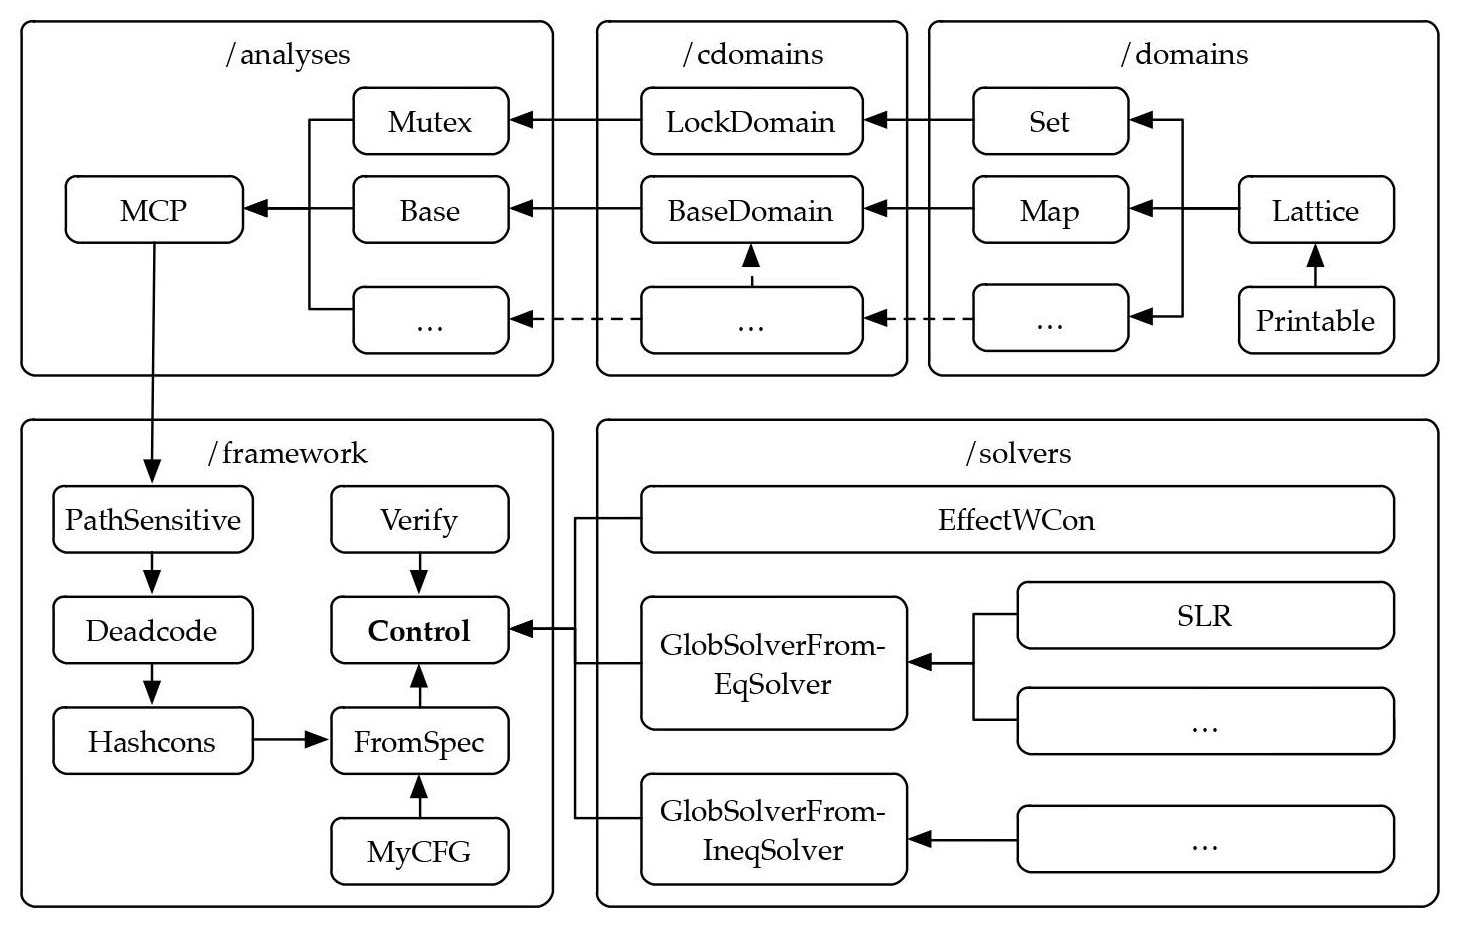
\includegraphics{../figures/goblint_structure_detailed.jpg}
    \caption{Schematic directory structure of \gob. Adapted from \parencite{apinis2014frameworks}}
    \label{fig:gob_structure_detail}
  \end{figure}

    \subsection{Taint analysis}\label{sec:implTaint}
      To define an analysis the \gob\ analyzer provides an interface, where the most relevant parts can be seen in \autoref{fig:analysis_interface}. This interface requires two modules \texttt{D} and \texttt{C} which define the domain and the context-sensitive part of the domain. It also requires the following functions: 
      \begin{itemize}
        \item \texttt{name} to uniquely refer to an analysis.
        \item \texttt{startstate} to define the state used when entering the analysis (similar to $\textsf{init}^{\#}$ from \autoref{chapter:background}).
        \item \texttt{query} to implement the query system of \gob. This allows an analysis to broadcast information to be used in analyses.
        \item \textit{Transfer functions} which define the abstract effects of actions (similar to $[\![A]\!]^{\#}$ from \autoref{chapter:background}).
        \item \textit{Functions for interprocedural analysis}
        \item \textit{Function for the analysis of multithreaded programs}
      \end{itemize}

      For our taint analysis we create a new module implementing this interface.\\
      As a \texttt{name} for \gob\ internally we chose \texttt{taintPartialContexts} because \texttt{taint} was already used, and the \texttt{name} needs to be unique. Let us now explain in detail how our new analysis module implements the given interface:

      \begin{figure}
        \centering
        \lstinputlisting[language={[Objective]Caml}, breaklines=true, breakatwhitespace=true]{../code/analyses.ml}
        \caption{Simplified Interface for implementing analyses in \gob}
        \label{fig:analysis_interface}
        %TODO: reference github for this file
      \end{figure}

      \subsubsection{Domain}
        We need to choose the domain \texttt{D} and the context domain \texttt{C}. According to the concept of our analysis described in \autoref{sec:formalTaint} the domain should be a set of variables. However, we are now analyzing the C language instead of our toy language. In C not every left-hand side of an assignment is just a simple variable, but can be one of many more complex thing, e.g., the memory location \texttt{*xptr} pointed to by the pointer \texttt{xptr}, the fourth place \texttt{a[3]} in an array \texttt{a}, the member \texttt{frac.n} of a struct \texttt{frac} and many more. All these options are described by a concept called \ac{lval}. There is an implementation of this type provided by \gob\ in the \texttt{Lval.CilLval} module. To be as precise as possible we use a set of \ac{lval}s instead of a set of variables for the implementation of the taint analysis.\\
        Another point worth mentioning is that we sometimes need the notion of "all variables" (or rather "all \ac{lval}s") when we want to express that everything is tainted. While conceptually using the full set $X$ poses no issue, in a concrete implementation this is extremely impractical and not even realizable if the set is infinitely large. For this case \gob\ provides a parametrized domain \texttt{ToppedSet(Base)}. This domain is either a set of elements of the \texttt{Base} type or alternatively a \texttt{Top} element which can be interpreted as the "full set of all \texttt{Base} elements". Therefore, we finally have \texttt{D = ToppedSet(Lval.CilLval)} for our domain. Note that this also defines the ordering on the domain to be the regular subset ordering.\\
        It remains to define the module \texttt{C}: We noted in \autoref{sec:formalTaint} that our analysis by itself is context insensitive. Therefore, the context domain of our analysis \texttt{C} is empty, which is expressed with the \texttt{Unit} domain provided by \gob. Note here, that this does not mean that the taint analysis is always performed context insensitively, i.e., it is only performed once per function. Since \gob\ uses a compound domain, there may be other context-sensitive analyses, forcing the whole compound analysis to analyze a function multiple times. Our taint analysis however never contributes differing sub contexts to the compound context.

      \subsubsection{The \texttt{startstate} function}
        This function computes the initial state for our analysis similar to the $\textsf{init}^{\#}$ function we introduced in \autoref{chapter:background}. As discussed in \autoref{sec:formalTaint}, we implement this function so that it returns the empty set.\\
        We note here however, that in practice we do not use the way, \texttt{startstate} is implemented in the scope of our thesis. In \gob\ this function is called before the main function is even entered. Thus, \texttt{enter} (which we define later) is still used to compute the entry state for the main function. We chose to implement \texttt{startstate} in this way for consistency.

      \subsubsection{Transfer functions}
        These functions implement the effect of actions on the state, similar to the abstract effects of actions $[\![A]\!]^{\#}$ in \autoref{chapter:background}. Variable declarations are handled by \texttt{vdecl} while \texttt{branch} handles checks for if-statements and loops. For these two actions our analysis just propagates the state from before, so the two mentioned functions use the default implementation from the \texttt{Analysis.IdentitySpec} of \gob. The default implementations of \texttt{Analysis.IdentitySpec} propagate the given state without change for any action.\\
        Much more interesting is the case of the \texttt{assign} function which handles the effect of an assignment to an \ac{lval}. For this case we want to add the \ac{lval} to our tainted set. The parameters for the \texttt{assign} function are: \texttt{ctx} which amongst other things contains the state from before, the \ac{lval} to which a value is assigned and an expression that evaluates to this value that is assigned. We are only interested in \texttt{ctx} and the \ac{lval}, as for the taint analysis only the fact that a value is assigned is relevant and not its concrete value.\\
        Tainting \ac{lval}s is not as straightforward as it might seem at first. Just adding it to the state from before, i.e., the tainted set, only suffices if the \ac{lval} is a specific location in the memory, e.g., a specific (local or global) variable. The \ac{lval} could however also be a reference to a location in the memory, e.g., a pointer. For these it is not helpful to just taint the reference because we need to know the specific memory locations that are or could be tainted. To solve this issue we make use of \gob's \texttt{MayPointTo} query. This takes a reference to the memory and asks all other activated analyses if they have any information about where this reference may point to. Just like everything else in the static analyzer \gob, the answer is an overapproximation, so we can be sure not to miss any location that could be referenced.\\
        In conclusion, tainting an \ac{lval} goes as follows: If the \ac{lval} is a specific memory location, this \ac{lval} is added to the tainted set. If it is a reference to the memory described by some expression, send a \texttt{MayPointTo} query to ask other analyses which memory locations this expression may point to and add the returned set of \ac{lval}s to the tainted set. We implemented this functionality in a helper function \texttt{taint\_lval}. Therefore, calling this function is the only thing the \texttt{assign} function needs to do as seen in \autoref{fig:assign}.

        \begin{figure}
          \centering
          \lstinputlisting[language={[Objective]Caml}]{../code/assign.ml}
          \caption{Implementation of the helper \texttt{taint\_lval} and the \texttt{assign} function}
          \label{fig:assign}
          %TODO: reference github for this file
        \end{figure}

      \subsubsection{Functions for interprocedural analysis}
        Here we define the functions \texttt{context}, \texttt{enter} and \texttt{combine}. These functions work similar to their abstract counterparts as described in \autoref{chapter:background}. In addition to these known functions, the interface also requires two additional functions: \texttt{return} which handles return statements right before a function is left and \texttt{special} which handles calls to library functions or other functions, for which we do not have the source code we can analyze.\\
        Our implementation does not differ a lot from the proposed formal description in \autoref{sec:formalTaint}. Since we are analyzing C and not our toy language, the only major difference is that we need to handle return values and function arguments. Therefore, we implement these functions as follows:

          \paragraph{\texttt{context}:} Our context domain is the \texttt{Unit} domain, and we do not want to generate different contexts for this analysis. Thus, this function always returns the unit element. 

          \paragraph{\texttt{enter}:} Like we discussed in \autoref{sec:formalTaint}, this function always returns the empty set, which is the entry state for the called function.

          \paragraph{\texttt{combine}:} The \texttt{combine} function first checks if there is an \ac{lval} to which the return value is assigned. If so, it taints this respective \ac{lval} in the caller state using the helper function \texttt{taint\_lval} introduced in the "Transfer Functions" section. After that it computes the union of the resulting state with the returned callee state and returns it.\\
          Summarized, the result of this function is the union of both states it receives for combining. It additionally adds \ac{lval}s which are possibly tainted by the return value.

          \paragraph{\texttt{return}:} In our formal description in \autoref{sec:formalTaint}, the $\textsf{combine}^{\#}_\textsf{t}$ function removed variables unreachable by the caller. In the concrete implementation, we give this functionality to the \texttt{return} function, so the removal happens right before the combine. We also remove function arguments as these are unreachable by the caller similar to local variables.
          It is worth pointing out that we do not just remove all \ac{lval}s corresponding to local variables or arguments. A function might exist multiple times in the current call stack, e.g., when the function is recursive. This can result in the existence of multiple versions of the same local variable. \gob\ treats these as being the same variable. Thus, when we remove a local variable we risk also removing a different version of it lower in the call stack, for which we still need the taintedness information. To address this issue, \texttt{return} sends an \texttt{IsMultiple} query for each variable to be removed and only removes those, that surely not have multiple versions. This query is already provided by \gob.

          \paragraph{\texttt{special}:} This function addresses library functions or other functions, for which we do not have the source code to analyze. The simple way to handle these, is to just return Top, i.e., saying "everything could be tainted", after a special call.\\
          This is how we handle unknown functions, however \gob\ provides "Library Descriptors", which contain information about some known C library functions, e.g., \texttt{printf}, \texttt{malloc}, \texttt{cos}, etc. With the respective Library Descriptor of a function, we can gain information about which addresses are "shallowly" written and which are "deeply" written by the call. Shallowly written addresses point to \ac{lval}s which might be directly written. Deeply written addresses however point to \ac{lval}s where not only the \ac{lval} itself, but possibly anything it might recursively point to could be written. Therefore, the \texttt{special} function makes use of \gob's \texttt{MayPointTo} and \texttt{ReachableFrom} queries in the following way:\\
          First the function checks if a Library Descriptor is available. If not, Top is returned. Otherwise, the shallowly and deeply written addresses are obtained from the Descriptor. Consequently, the union of 
          \begin{itemize}
            \item the state before the call
            \item anything that is possibly tainted by the return value (using \texttt{taint\_lval} like in \texttt{combine}) 
            \item the set of \ac{lval}s returned by the \texttt{MayPointTo} query for any shallowly written address
            \item the set of \ac{lval}s returned by the \texttt{ReachableFrom} query for any deeply written address
          \end{itemize}
          is returned by the \texttt{special} function.

      \subsubsection{Function for the analysis of multithreaded programs}
        To be able to analyze multithreaded programs, \gob's analysis interface requires the following functions: \texttt{threadenter} to compute the startstate for the newly created thread and \texttt{threadspawn} which computes the effect of a thread creating instruction to the state of the creating thread.\\
        We implement the former of these two functions similarly to our \texttt{startstate} and \texttt{enter}. Thus, \texttt{threadenter} returns the empty set.\\
        To implement the other function, \texttt{threadspawn}, we consider how a thread creation effects the state of the creator. We note that for our notion of taintedness the only relevant effect is, that the thread creating function may write thread ID variables to which it receives a reference as an argument. Thus, this function uses the helper function \texttt{taint\_lval} defined in the "Transfer Functions" section to add possibly tainted \ac{lval}s to the state from before and returns the result.

      \subsubsection{The \texttt{query} function}
        We want to enable our taint analysis to tell other analyses which \ac{lval}s are tainted at a specific program point. Therefore, we add a new query \texttt{MayBeTainted} to the query system of \gob. The result of this query should be a set containing \ac{lval}s which may be tainted, i.e., any \ac{lval} that is not in the returned set is definitely untainted.\\
        After this addition we are able to make our \texttt{taintPartialContexts} analysis answer to this query. Therefore, our analysis implements the \texttt{query} function in such a way that it answers only to \texttt{MayBeTainted} queries with the current state but does not answer other queries.

    \subsection{Benefiting other analyses}\label{sec:improveVariableAnalyses}
    In this section we discuss how we improved other existing analyses in \gob\ using the taint analysis we implemented in \autoref{sec:implTaint}.
    \subsubsection{Improving the \texttt{base} analysis}
      The main analysis that benefits from the taint analysis is the \texttt{base} analysis of \gob. This analysis implements a very much extended approach of the basic values-of-variables analysis we formally defined in \autoref{chapter:background}. The \texttt{base} analysis is however still based on the main goal and basic concept of finding a mapping from program variables to possible values at each program point. Therefore, this analysis uses a mapping from variables to their possible values as part of its domain. However, here the \texttt{ValueDomain} of the mapping is much more complex than just a set of possible integers. It provides abstractions for virtually any type in C, including arrays, structs and pointers. Even more though, the \texttt{ValueDomain} is highly configurable. Amongst other options it allows choosing between different ways of abstracting integer values or arrays. One interesting option related to the topic of this thesis is the possibility to choose between different degrees of context sensitivity: the analysis can be fully context-sensitive, insensitive with respect to integer variables (abstracted by intervals or in general), only sensitive with respect to pointers or completely insensitive. When choosing anything but the completely context-sensitive option, this analysis experiences the (avoidable) loss of precision described in \autoref{sec:precisionLoss}.\\
      To reduce this loss we need to change the \texttt{combine} function of the \texttt{base} analysis so that it uses the results of our \texttt{taintPartialContexts} analysis. Let us first describe how the \texttt{combine} function was implemented before our changes:
      \begin{enumerate}
        \item The return value is saved. Its value is removed from the callee state.
        \item All globals are removed from the caller state.
        \item Everything from the callee state is added to the caller, possibly overwriting caller values. This excludes the return value which is handled separately.
        \item Some further adjustments according to the configuration are performed to the resulting state.
        \item The saved return value is added to the state before it is returned.
      \end{enumerate}
      To implement our changes we will focus on the steps 2 and 3, where the caller mapping is updated. The other steps will remain the same.\\
      The core idea to implement the concept proposed in \autoref{sec:formalImprove} is as follows: First we get the set of possibly tainted \ac{lval}s from the callee. We then iterate over its elements one by one, where for each tainted \ac{lval} we update the caller mapping with the corresponding value from the callee mapping, i.e., we get the value corresponding to that \ac{lval} from the callee mapping and set the \ac{lval} to map to this value in the caller mapping. This functionality of updating the caller mapping with the callee mapping using the tainted set is implemented in a helper function \texttt{combine\_st}.\\
      Before we explain how this helper function is implemented, we first show how it is embedded in the current implementation of the \texttt{combine} function. As discussed, we alter steps 2 and 3: First we send a \texttt{MayPointTo} query to the return state of the callee. We then check if the query returned the Top set, i.e., the notion that everything is tainted. In this case we perform the unchanged steps 2 and 3 just like before. Amongst other cases, this can happen, when the \texttt{base} analysis is run without our taint analysis being activated.\\
      Let us now define what happens, when the result of the query is an explicit set. Before calling the helper function \texttt{combine\_st}, we need to handle two special cases here:
      \begin{itemize}
        \item For a global variable, there is no mapping in the callee state, but there is one in the caller state. This case can occur in multithreaded mode, if this variable was protected by a mutex before the call, but the mutex was released in the called function. In this case, the mapping for this variable would be removed from the state within the callee. In the \texttt{combine} function, we do need to keep this new information from the callee for such a variable, i.e., remove it from the caller mapping. Therefore, we filter over the caller mapping and remove all globals, for which there exists no mapping in the callee mapping.

        \item For a global variable, there is a mapping in the callee state, but there is none in the caller state. This case can occur if new information is gained within the call, e.g., some new memory is allocated. This information is not tracked by the tainted set and would therefore not be copied into the caller state. Since we still want to have this new information after the combine, we add all these mappings from the callee to the caller.
      \end{itemize}
      These cases have to be handled separately, as for these the corresponding \ac{lval} is not necessarily contained in the tainted set. After the two special cases are handled, we use the \texttt{combine\_st} helper function to finally update the tainted \ac{lval}s in the caller state. We then proceed with the resulting state to the steps 4 and 5 like before.\\
      We note here that we added a new parameter \texttt{f\_ask} to the \texttt{combine} function. To do this we had to update the analysis interface and consequently all analyses implementing it. This new parameter allows us to send queries to the returned callee state, which was not possible before.
      \paragraph{\texttt{combine\_st}:} This helper function takes the caller state (updated according to the two special cases), the callee state and the set of tainted \ac{lval}s. The difficulty here is, that while the tainted set is a set of \ac{lval}s, the mappings from the states of the \texttt{base} analysis are mappings from variables to abstractions of their possible values. This means, that our tainted set may include specific places in an array or specific members of a struct, e.g., \texttt{a[3]} and \texttt{frac.n}. In contrast to this, the mappings we want to combine do not map \texttt{a[3]} and \texttt{frac.n} to abstract values, but rather map \texttt{a} to some abstraction of an array and \texttt{frac} to some abstraction of a struct. To solve this issue we make use of the \texttt{get} and \texttt{set\_savetop} functions provided by the module of the \texttt{base} analysis. These functions allow us to get and set values of addresses to specific \ac{lval}s in a variable mapping of the \texttt{base} analysis.\\
      Therefore, the implementation of this function goes as follows: We fold over the tainted set. For each \ac{lval} we build an address to this \ac{lval}. Then we try to \texttt{get} the value this address points to from the callee state. If this returns a value, we use \texttt{set\_savetop} to update the caller state, i.e., set the address to the value we got. Otherwise, we proceed with the next \ac{lval}.\\
      There are however a few special cases to handle: One issue is that in \gob\ there exists a domain for abstracting array values called "partitioned array". This abstraction saves an index which it uses to split an array into three parts: The group of all values to the left of the index, the value at the index itself and the group of all values to the right. Each of the three parts is abstracted with a collective value. The index can be either a specific integer or a variable.\\
      For array variables abstracted with this "partitioned array" domain, copying \ac{lval}s one by one does not work, as the information of the partitioning is lost when we attempt it. Therefore, we check if the current value corresponds to a place in an array abstracted with the "partitioned array" domain and if so, we copy the whole partitioned array from the callee mapping to the caller mapping.\\
      A similar issue occurs with values of void type, as for these the \texttt{get} does not work correctly. Therefore, we get the value for the corresponding variable from the callee mapping itself and update the caller mapping with it.\\
      The last issue we need to address is again related to partitioned arrays. Recall, that an array can be partitioned by the value of a variable. This means, that if a variable is tainted which is used as a partitioning index, the partitioned array in the caller mapping is invalid. Therefore, for each \ac{lval} we check if it corresponds to a variable partitioning an array. If so, we update the caller state by copying all abstracted arrays which are partitioned by the variable in question from the callee mapping to the caller mapping. This is possible, because the state of the \texttt{base} analysis keeps track of which arrays are partitioned by certain variables.\\
      Finally, after we are done folding over all tainted \ac{lval}s, the function returns the modified caller state.
      %TODO: Summarize the updated combine

    \subsubsection{Improving other Variable Analyses}
      In \gob\ there are multiple other analyses which can be described by our notion of a variable analysis. For some of these we are able to the precision loss of partial contexts by using the results from our \texttt{taintPartialContexts} analysis. Let us briefly discuss the details of these improvements:

      \paragraph{The \texttt{varEq} analysis:}\mbox{}\\
        This analysis tracks, which \ac{lval}s definitely hold the same value, irregardless of what this value is. As an example, after an assignment \texttt{a[3] = y;} this analysis propagates the information that \texttt{a[3]} and \texttt{y} in an equality set, until either \texttt{a[3]} or \texttt{b} are written.\\
        One can construct a case, where a function \texttt{f()} is called twice, once where some equality \texttt{x = y} holds and once where it does not hold. We assume that \texttt{x} and \texttt{y} are not altered within \texttt{f()}. If the \texttt{varEq} analysis is performed context-insensitively, we would lose the equality information when the \texttt{combine} is performed after both calls. This is because the equality information is discarded when the entry states are joined.\\
        So far, the \texttt{combine} function just propagated the callee return state. This can be improved in the following way: We obtain the tainted set and remove all equality sets containing at least one tainted \ac{lval} from the caller state. Then we compute the greatest lower bound of the resulting caller state and the callee state. This means, we compute a state that unifies the information from the caller state without tainted \ac{lval}s with the information from the callee state.\\
        In the example from above this changed \texttt{combine} allows us to keep the equality \texttt{x=y} when the taint analysis is activated.

      \paragraph{The \texttt{relation} analysis:}\mbox{}\\
        This analysis tracks relations between variables. The analysis can be configured to use different kinds of relations implemented in different domains. An example for these domains is the octagon domain, which works with relations of the form $\langle x \rangle + \langle y \rangle \geq 0$, where $\langle x \rangle$ stands for either $x$ or $-x$. The relation analysis is parametrized in such a way that our changes apply to the analysis independent of the selected relation domain.\\
        The case where this analysis unnecessarily loses precision because of context insensitivity, is similar to the one discussed in the paragraph discussing the improvement of the \texttt{varEq} analysis: A function \texttt{f()} is called twice, where some relation between the variables \texttt{x} and \texttt{y} once holds and once does not hold. When the entry states for both calls are joined, the relation in question is removed and is therefore missing after the call. We once again assume that \texttt{x} and \texttt{y} are not altered within \texttt{f()}.\\
        Before we apply our changes, the \texttt{combine} function of the \texttt{relation} analysis is implemented so that it removes all information related to global variables from the caller state and merges the result with the callee state. The result contains the relations from the caller that are not related to globals and all relations from the callee.\\
        Accessing the result of our taint analysis via a query, we can improve this way of combining. We achieve this by only removing relations related to tainted global variables and keep those that only relate to locals and untainted globals. After that, the result is merged with the callee state like before.\\
        We note here, that this analysis tracks relations between variables while our tainted set contains tainted \ac{lval}s. Therefore, we convert the set of tainted \ac{lval}s to a set of tainted variables. This is easily possible, since all \ac{lval}s in our tainted set refer to variables or specific parts of variables. In particular, they do not point to some memory location, which would make identifying a corresponding variable difficult.

      \paragraph{The \texttt{condVars} analysis:}\mbox{}\\
        This analysis tracks equalities between variables and logical expressions. Take the following statement as an example: \texttt{tv = (c == 0);}. For this statement, the \texttt{condVars} analysis tracks, that the variable \texttt{tv} holds the value of the logical expression \texttt{c == 0}. This information can be used, when there is an \texttt{if} statement, checking whether \texttt{tv} is true or not. Knowing \texttt{tv} is equal to \texttt{c == 0}, this analysis can provide the information that \texttt{c == 0} evaluates to \texttt{true} in the \texttt{true}-branch of the \texttt{if} statement.\\
        Currently, the \texttt{combine} function of this analysis is implemented to discard the callee return state and remove all information related to global variables from the caller state. This results in the loss of all information related to globals whenever a function is called, irregardless whether the \texttt{condVars} analysis is performer context sensitively or insensitively.\\
        We can improve this by only removing information related to tainted globals from the caller state and keeping information related to untainted globals. This makes the \texttt{condVars} analysis more precise whenever the \texttt{taintPartialContexts} analysis is activated. Again we note here, that this analysis is concerned with information related to variables, not \ac{lval}s. Therefore, we convert the set of tainted \ac{lval}s to a set of tainted variables like in the previous paragraph. 
      